\section{Introduction}
\label{sec:intro}

How close each part of a hand is to the object it manipulates, before, during and after contact, is a compact description of manipulation that robot learning, augmented-reality interfaces and activity understanding can consume directly. ARCTIC~\cite{fan2023arctic} formalised this quantity as an \emph{interaction field}, the distance from every point of one shape to the closest point of the other, and TACO~\cite{liu2024taco} extended it to tool use. SHOW3D~\cite{rim2026show3d} brought the problem into the wild with 4.3\,M frames of hands manipulating 21 objects in more than 30 indoor and outdoor locations, annotated in three dimensions by an ego-exo capture rig. Its HANDS@ECCV~2026 challenge asks for a joint-anchored version of the field: for each of the 21 UmeTrack landmarks~\cite{han2022umetrack} of each hand, the three-dimensional vector to the nearest vertex of the object mesh, estimated from two synchronised egocentric views of a Meta Quest~3 headset~\cite{rim2026show3dapi} (\cref{fig:teaser}).

\begin{figure*}[t]
\centering
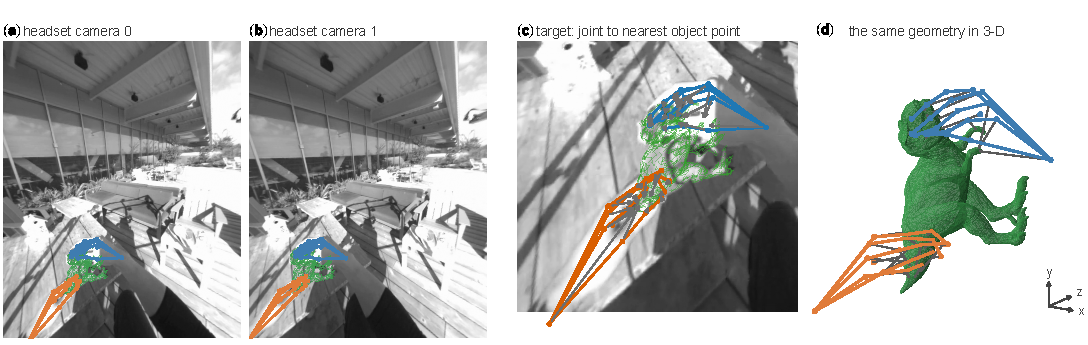
\includegraphics[width=\textwidth]{../figures/fig1_teaser.pdf}
\caption{The joint-anchored interaction field on a held-out SHOW3D frame. (a, b) The two synchronised headset views with the ground-truth skeletons (left hand orange, right hand blue) and the posed object mesh (green wireframe). (c) The reference view cropped around the interaction; every grey arrow is the target vector from a joint to the nearest point of the posed mesh. (d) The same joints, mesh and vectors in three dimensions: the 21 endpoints of each hand lie on one rigid surface, which is the structure the proposed model exploits.}
\label{fig:teaser}
\end{figure*}

The challenge produced strong systems. GOLF~\cite{zou2026golf} adapts a DINOv3 ViT-H+~\cite{simeoni2025dinov3} with low-rank adaptation (LoRA)~\cite{hu2022lora}, samples region tokens around the hands and the object, tags every token with the Pl\"ucker coordinates of its viewing ray and decodes 42 joint queries into vectors; JSSR~\cite{jin2026jssr} adds temporal context and an epipolar search for the field endpoints. Between the official ResNet-50 baseline and GOLF, the hidden-test error fell from 59 to 28\,mm. GOLF's own submission trace is instructive: most of the gain came from the backbone (5.7\,mm from ViT-L to the adapted ViT-H+) and from local detail (2.7\,mm), whereas adding the second view changed the error by 0.19\,mm and ray encoding by 0.6\,mm~\cite{zou2026golf}. With a 64\,mm baseline and hands at 200 to 400\,mm, one pixel of disparity corresponds to 1.4 to 5.5\,mm of depth, so stereo is geometrically informative; the small empirical gain suggests either that the remaining error is not primarily a depth error, or that direct regression does not exploit the geometry it is given. Nobody has reported where the remaining 28\,mm come from.

This paper starts from an observation about the target rather than the architecture. The field is a deterministic function of three quantities: the hand joints, the six-degree-of-freedom pose of the object, and the object mesh. All three are supervised in the training set, the mesh is a fixed asset shipped with the benchmark, and the object category is provided at test time. Yet every published solution regresses the 126 numbers directly and ignores that the 21 endpoints of a hand lie on one rigid surface. The same structure has long been exploited in the contact literature, where proximity is derived from posed hand and object geometry rather than estimated from pixels~\cite{yang2021cpf,grady2021contactopt,qi2024hoisdf,chen2023gsdf,ilic2026egophi}; the interaction field is exactly such a derived quantity.

We therefore propose \emph{factored interaction fields} (\method{}): a transformer decoder over frozen DINOv3 tokens of both views that predicts camera-frame hand joints and the object pose, evaluates the field through a differentiable soft nearest-vertex operator on the posed mesh, and fuses this geometric estimate with a direct regression head using per-joint predicted precisions. The geometric head yields fields whose endpoints lie on the object by construction and is invariant to object symmetries; the direct head remains a fallback where the pose is not observable; the fusion is a likelihood-weighted average rather than a learned gate or an ensemble. Because the factored model exposes its intermediate quantities, it also enables an analysis the field itself does not permit: swapping predicted and ground-truth joints or object poses decomposes the error into hand and object components, and stratifying by field magnitude, joint visibility and observability shows which frames drive the mean.

We evaluate under a deliberately controlled protocol. The evaluation server is closed and the test labels are withheld, so all experiments use subject-level splits of the training subjects; all token-based models share one frozen backbone, one feature cache, one decoder and one optimiser, so that differences are attributable to the factorisation alone; the main comparison is repeated on two disjoint pairs of held-out subjects and with two seeds; and the falsification criterion was fixed before any model was trained: the hypothesis is rejected if the factored model does not beat the direct head on the mean error at a matched representation, \emph{and} is not better on far-field or occluded joints, \emph{and} does not transfer better to a second dataset. We also build HOT3D-IF, a joint-level version of the task on HOT3D~\cite{banerjee2025hot3d}, whose objects, hand skeleton and headset SHOW3D shares, by rectifying its fisheye streams and recovering landmarks through UmeTrack forward kinematics.

The results support the first two clauses and refute the third, and the analysis of the trained models turns out to be more informative than the headline number. \method{} lowers the error of the matched direct regressor from 46.2 to 44.4\,mm on the official development subjects (two seeds each, ranges not overlapping) and from 35.7 to 34.1\,mm on a second subject pair, against 60.5\,mm for the official baseline. A single-view \method{} at 45.2\,mm outperforms the two-view direct model. The gain rises with difficulty, from 0.6\,mm for joints within 15\,mm of the object to 3.0\,mm beyond 60\,mm and 21\,mm when the hand leaves the image. Inside the model, however, the improvement is carried by the direct head, whose representation is shaped by the geometric supervision: inference-time fusion contributes 0.1\,mm, the geometric head alone is 11\,mm worse than the direct head, and its predicted scale saturated at the clamp in four of the five precision-fusion runs we inspected. The object pose, not the hand, is the bottleneck of the geometric route in domain, and the hand becomes the bottleneck out of domain. The advantage does not transfer to HOT3D in any of four cross-dataset settings and disappears when HOT3D frames are added to training. We report these findings as they are, because they bound what a factored representation can be expected to deliver and where the remaining error actually sits.

Our contributions are:
(i) a factored formulation of joint-anchored interaction fields with a differentiable nearest-vertex operator, closed-form differentiable object pose and precision-weighted fusion with direct regression (\cref{sec:method});
(ii) a controlled evaluation at a fixed frozen representation on two held-out subject pairs, with a stratified analysis showing that the gain concentrates in far-field, occluded and out-of-view joints (\cref{sec:results});
(iii) an analysis of the trained models, including oracle swaps of the geometric arguments and the calibration of the learned precisions, which locates the gain in the shared representation rather than in the fusion (\cref{sec:inside});
(iv) HOT3D-IF, a joint-level cross-dataset protocol between SHOW3D and HOT3D, and the finding that the factored advantage does not transfer (\cref{sec:cross}).
All experiments run on a single laptop with 16\,GB of unified memory; code, configurations, derived labels and every trained checkpoint are released.
